\documentclass[1p]{elsarticle_modified}
%\bibliographystyle{elsarticle-num}

%\usepackage[colorlinks]{hyperref}
%\usepackage{abbrmath_seonhwa} %\Abb, \Ascr, \Acal ,\Abf, \Afrak
\usepackage{amsfonts}
\usepackage{amssymb}
\usepackage{amsmath}
\usepackage{amsthm}
\usepackage{scalefnt}
\usepackage{amsbsy}
\usepackage{kotex}
\usepackage{caption}
\usepackage{subfig}
\usepackage{color}
\usepackage{graphicx}
\usepackage{xcolor} %% white, black, red, green, blue, cyan, magenta, yellow
\usepackage{float}
\usepackage{setspace}
\usepackage{hyperref}

\usepackage{tikz}
\usetikzlibrary{arrows}

\usepackage{multirow}
\usepackage{array} % fixed length table
\usepackage{hhline}

%%%%%%%%%%%%%%%%%%%%%
\makeatletter
\renewcommand*\env@matrix[1][\arraystretch]{%
	\edef\arraystretch{#1}%
	\hskip -\arraycolsep
	\let\@ifnextchar\new@ifnextchar
	\array{*\c@MaxMatrixCols c}}
\makeatother %https://tex.stackexchange.com/questions/14071/how-can-i-increase-the-line-spacing-in-a-matrix
%%%%%%%%%%%%%%%

\usepackage[normalem]{ulem}

\newcommand{\msout}[1]{\ifmmode\text{\sout{\ensuremath{#1}}}\else\sout{#1}\fi}
%SOURCE: \msout is \stkout macro in https://tex.stackexchange.com/questions/20609/strikeout-in-math-mode

\newcommand{\cancel}[1]{
	\ifmmode
	{\color{red}\msout{#1}}
	\else
	{\color{red}\sout{#1}}
	\fi
}

\newcommand{\add}[1]{
	{\color{blue}\uwave{#1}}
}

\newcommand{\replace}[2]{
	\ifmmode
	{\color{red}\msout{#1}}{\color{blue}\uwave{#2}}
	\else
	{\color{red}\sout{#1}}{\color{blue}\uwave{#2}}
	\fi
}

\newcommand{\Sol}{\mathcal{S}} %segment
\newcommand{\D}{D} %diagram
\newcommand{\A}{\mathcal{A}} %arc


%%%%%%%%%%%%%%%%%%%%%%%%%%%%%5 test

\def\sl{\operatorname{\textup{SL}}(2,\Cbb)}
\def\psl{\operatorname{\textup{PSL}}(2,\Cbb)}
\def\quan{\mkern 1mu \triangleright \mkern 1mu}

\theoremstyle{definition}
\newtheorem{thm}{Theorem}[section]
\newtheorem{prop}[thm]{Proposition}
\newtheorem{lem}[thm]{Lemma}
\newtheorem{ques}[thm]{Question}
\newtheorem{cor}[thm]{Corollary}
\newtheorem{defn}[thm]{Definition}
\newtheorem{exam}[thm]{Example}
\newtheorem{rmk}[thm]{Remark}
\newtheorem{alg}[thm]{Algorithm}

\newcommand{\I}{\sqrt{-1}}
\begin{document}

%\begin{frontmatter}
%
%\title{Boundary parabolic representations of knots up to 8 crossings}
%
%%% Group authors per affiliation:
%\author{Yunhi Cho} 
%\address{Department of Mathematics, University of Seoul, Seoul, Korea}
%\ead{yhcho@uos.ac.kr}
%
%
%\author{Seonhwa Kim} %\fnref{s_kim}}
%\address{Center for Geometry and Physics, Institute for Basic Science, Pohang, 37673, Korea}
%\ead{ryeona17@ibs.re.kr}
%
%\author{Hyuk Kim}
%\address{Department of Mathematical Sciences, Seoul National University, Seoul 08826, Korea}
%\ead{hyukkim@snu.ac.kr}
%
%\author{Seokbeom Yoon}
%\address{Department of Mathematical Sciences, Seoul National University, Seoul, 08826,  Korea}
%\ead{sbyoon15@snu.ac.kr}
%
%\begin{abstract}
%We find all boundary parabolic representation of knots up to 8 crossings.
%
%\end{abstract}
%\begin{keyword}
%    \MSC[2010] 57M25 
%\end{keyword}
%
%\end{frontmatter}

%\linenumbers
%\tableofcontents
%
\newcommand\colored[1]{\textcolor{white}{\rule[-0.35ex]{0.8em}{1.4ex}}\kern-0.8em\color{red} #1}%
%\newcommand\colored[1]{\textcolor{white}{ #1}\kern-2.17ex	\textcolor{white}{ #1}\kern-1.81ex	\textcolor{white}{ #1}\kern-2.15ex\color{red}#1	}

{\Large $\underline{10_{77}~(K10a_{18})}$}

\setlength{\tabcolsep}{10pt}
\renewcommand{\arraystretch}{1.6}
\vspace{1cm}\begin{tabular}{m{100pt}>{\centering\arraybackslash}m{274pt}}
\multirow{5}{120pt}{
	\centering
	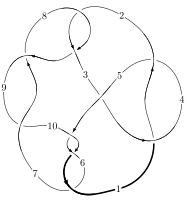
\includegraphics[width=112pt]{../../../GIT/diagram.site/Diagrams/png/161_10_77.png}\\
\ \ \ A knot diagram\footnotemark}&
\allowdisplaybreaks
\textbf{Linearized knot diagam} \\
\cline{2-2}
 &
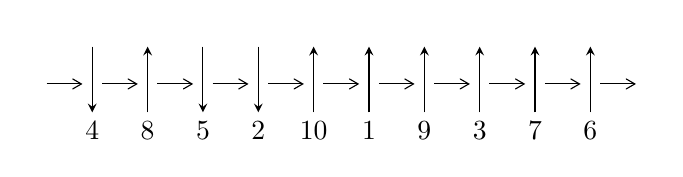
\begin{tikzpicture}[x=20pt, y=17pt]
	% nodes
	\node (C0) at (0, 0) {};
	\node (C1) at (1, 0) {};
	\node (C1U) at (1, +1) {};
	\node (C1D) at (1, -1) {4};

	\node (C2) at (2, 0) {};
	\node (C2U) at (2, +1) {};
	\node (C2D) at (2, -1) {8};

	\node (C3) at (3, 0) {};
	\node (C3U) at (3, +1) {};
	\node (C3D) at (3, -1) {5};

	\node (C4) at (4, 0) {};
	\node (C4U) at (4, +1) {};
	\node (C4D) at (4, -1) {2};

	\node (C5) at (5, 0) {};
	\node (C5U) at (5, +1) {};
	\node (C5D) at (5, -1) {10};

	\node (C6) at (6, 0) {};
	\node (C6U) at (6, +1) {};
	\node (C6D) at (6, -1) {1};

	\node (C7) at (7, 0) {};
	\node (C7U) at (7, +1) {};
	\node (C7D) at (7, -1) {9};

	\node (C8) at (8, 0) {};
	\node (C8U) at (8, +1) {};
	\node (C8D) at (8, -1) {3};

	\node (C9) at (9, 0) {};
	\node (C9U) at (9, +1) {};
	\node (C9D) at (9, -1) {7};

	\node (C10) at (10, 0) {};
	\node (C10U) at (10, +1) {};
	\node (C10D) at (10, -1) {6};
	\node (C11) at (11, 0) {};

	% arrows
	\draw[->,>={angle 60}]
	(C0) edge (C1) (C1) edge (C2) (C2) edge (C3) (C3) edge (C4) (C4) edge (C5) (C5) edge (C6) (C6) edge (C7) (C7) edge (C8) (C8) edge (C9) (C9) edge (C10) (C10) edge (C11) ;	\draw[->,>=stealth]
	(C1U) edge (C1D) (C2D) edge (C2U) (C3U) edge (C3D) (C4U) edge (C4D) (C5D) edge (C5U) (C6D) edge (C6U) (C7D) edge (C7U) (C8D) edge (C8U) (C9D) edge (C9U) (C10D) edge (C10U) ;
	\end{tikzpicture} \\
\hhline{~~} \\& 
\textbf{Solving Sequence} \\ \cline{2-2} 
 &
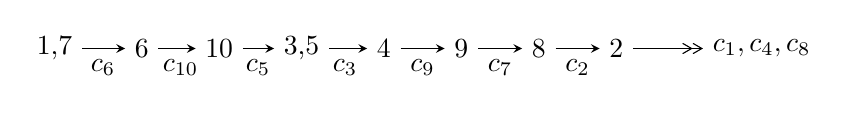
\begin{tikzpicture}[x=28pt, y=7pt]
	% node
	\node (A0) at (-1/8, 0) {1,7};
	\node (A1) at (1, 0) {6};
	\node (A2) at (2, 0) {10};
	\node (A3) at (49/16, 0) {3,5};
	\node (A4) at (33/8, 0) {4};
	\node (A5) at (41/8, 0) {9};
	\node (A6) at (49/8, 0) {8};
	\node (A7) at (57/8, 0) {2};
	\node (C1) at (1/2, -1) {$c_{6}$};
	\node (C2) at (3/2, -1) {$c_{10}$};
	\node (C3) at (5/2, -1) {$c_{5}$};
	\node (C4) at (29/8, -1) {$c_{3}$};
	\node (C5) at (37/8, -1) {$c_{9}$};
	\node (C6) at (45/8, -1) {$c_{7}$};
	\node (C7) at (53/8, -1) {$c_{2}$};
	\node (A8) at (9, 0) {$c_{1},c_{4},c_{8}$};

	% edge
	\draw[->,>=stealth]	
	(A0) edge (A1) (A1) edge (A2) (A2) edge (A3) (A3) edge (A4) (A4) edge (A5) (A5) edge (A6) (A6) edge (A7) ;
	\draw[->>,>={angle 60}]	
	(A7) edge (A8);
\end{tikzpicture} \\ 

\end{tabular} \\

\footnotetext{
The image of knot diagram is generated by the software ``\textbf{Draw programme}" developed by Andrew Bartholomew(\url{http://www.layer8.co.uk/maths/draw/index.htm\#Running-draw}), where we modified some parts for our purpose(\url{https://github.com/CATsTAILs/LinksPainter}).
}\phantom \\ \newline 
\centering \textbf{Ideals for irreducible components\footnotemark of $X_{\text{par}}$} 
 
\begin{align*}
I^u_{1}&=\langle 
u^{22}- u^{21}+\cdots+b-1,\;u^{22}-9 u^{20}+\cdots+a-1,\;u^{23}-2 u^{22}+\cdots- u+1\rangle \\
I^u_{2}&=\langle 
u^6-2 u^4+u^2+b,\;u^4- u^2+a+1,\;u^9-3 u^7- u^6+3 u^5+2 u^4+u^3- u^2-2 u-1\rangle \\
I^u_{3}&=\langle 
b,\;a-1,\;u+1\rangle \\
\\
\end{align*}
\raggedright * 3 irreducible components of $\dim_{\mathbb{C}}=0$, with total 33 representations.\\
\footnotetext{All coefficients of polynomials are rational numbers. But the coefficients are sometimes approximated in decimal forms when there is not enough margin.}
\newpage
\renewcommand{\arraystretch}{1}
\centering \section*{I. $I^u_{1}= \langle u^{22}- u^{21}+\cdots+b-1,\;u^{22}-9 u^{20}+\cdots+a-1,\;u^{23}-2 u^{22}+\cdots- u+1 \rangle$}
\flushleft \textbf{(i) Arc colorings}\\
\begin{tabular}{m{7pt} m{180pt} m{7pt} m{180pt} }
\flushright $a_{1}=$&$\begin{pmatrix}0\\u\end{pmatrix}$ \\
\flushright $a_{7}=$&$\begin{pmatrix}1\\0\end{pmatrix}$ \\
\flushright $a_{6}=$&$\begin{pmatrix}1\\u^2\end{pmatrix}$ \\
\flushright $a_{10}=$&$\begin{pmatrix}- u\\- u^3+u\end{pmatrix}$ \\
\flushright $a_{3}=$&$\begin{pmatrix}- u^{22}+9 u^{20}+\cdots+5 u+1\\- u^{22}+u^{21}+\cdots- u+1\end{pmatrix}$ \\
\flushright $a_{5}=$&$\begin{pmatrix}- u^2+1\\- u^4+2 u^2\end{pmatrix}$ \\
\flushright $a_{4}=$&$\begin{pmatrix}u^{22}- u^{21}+\cdots+6 u-1\\- u^{19}+7 u^{17}+\cdots-6 u^2- u\end{pmatrix}$ \\
\flushright $a_{9}=$&$\begin{pmatrix}u^3-2 u\\- u^3+u\end{pmatrix}$ \\
\flushright $a_{8}=$&$\begin{pmatrix}u^6-3 u^4+2 u^2+1\\- u^6+2 u^4- u^2\end{pmatrix}$ \\
\flushright $a_{2}=$&$\begin{pmatrix}- u^{21}+9 u^{19}+\cdots+15 u^2+6 u\\- u^{22}+u^{21}+\cdots- u+1\end{pmatrix}$\\&\end{tabular}
\flushleft \textbf{(ii) Obstruction class $= -1$}\\~\\
\flushleft \textbf{(iii) Cusp Shapes $= -2 u^{21}+4 u^{20}+18 u^{19}-32 u^{18}-70 u^{17}+100 u^{16}+148 u^{15}-132 u^{14}-164 u^{13}-4 u^{12}+38 u^{11}+200 u^{10}+130 u^9-148 u^8-136 u^7-68 u^6+2 u^5+80 u^4+50 u^3+20 u^2-6 u$}\\~\\
\newpage\renewcommand{\arraystretch}{1}
\flushleft \textbf{(iv) u-Polynomials at the component}\newline \\
\begin{tabular}{m{50pt}|m{274pt}}
Crossings & \hspace{64pt}u-Polynomials at each crossing \\
\hline $$\begin{aligned}c_{1},c_{4}\end{aligned}$$&$\begin{aligned}
&u^{23}-2 u^{22}+\cdots+3 u-1
\end{aligned}$\\
\hline $$\begin{aligned}c_{2},c_{8}\end{aligned}$$&$\begin{aligned}
&u^{23}-2 u^{22}+\cdots+2 u-2
\end{aligned}$\\
\hline $$\begin{aligned}c_{3}\end{aligned}$$&$\begin{aligned}
&u^{23}+12 u^{22}+\cdots+7 u+1
\end{aligned}$\\
\hline $$\begin{aligned}c_{5},c_{6},c_{10}\end{aligned}$$&$\begin{aligned}
&u^{23}+2 u^{22}+\cdots- u-1
\end{aligned}$\\
\hline $$\begin{aligned}c_{7},c_{9}\end{aligned}$$&$\begin{aligned}
&u^{23}-6 u^{22}+\cdots+8 u-4
\end{aligned}$\\
\hline
\end{tabular}\\~\\
\newpage\renewcommand{\arraystretch}{1}
\flushleft \textbf{(v) Riley Polynomials at the component}\newline \\
\begin{tabular}{m{50pt}|m{274pt}}
Crossings & \hspace{64pt}Riley Polynomials at each crossing \\
\hline $$\begin{aligned}c_{1},c_{4}\end{aligned}$$&$\begin{aligned}
&y^{23}-12 y^{22}+\cdots+7 y-1
\end{aligned}$\\
\hline $$\begin{aligned}c_{2},c_{8}\end{aligned}$$&$\begin{aligned}
&y^{23}-6 y^{22}+\cdots+8 y-4
\end{aligned}$\\
\hline $$\begin{aligned}c_{3}\end{aligned}$$&$\begin{aligned}
&y^{23}+32 y^{21}+\cdots+31 y-1
\end{aligned}$\\
\hline $$\begin{aligned}c_{5},c_{6},c_{10}\end{aligned}$$&$\begin{aligned}
&y^{23}-20 y^{22}+\cdots-9 y-1
\end{aligned}$\\
\hline $$\begin{aligned}c_{7},c_{9}\end{aligned}$$&$\begin{aligned}
&y^{23}+18 y^{22}+\cdots-8 y-16
\end{aligned}$\\
\hline
\end{tabular}\\~\\
\newpage\flushleft \textbf{(vi) Complex Volumes and Cusp Shapes}
$$\begin{array}{c|c|c}  
\text{Solutions to }I^u_{1}& \I (\text{vol} + \sqrt{-1}CS) & \text{Cusp shape}\\
 \hline 
\begin{aligned}
u &= -0.094963 + 0.875706 I \\
a &= \phantom{-}2.34528 + 0.84882 I \\
b &= -1.86529 - 0.93050 I\end{aligned}
 & -6.35503 - 7.52364 I & -0.34364 + 6.02284 I \\ \hline\begin{aligned}
u &= -0.094963 - 0.875706 I \\
a &= \phantom{-}2.34528 - 0.84882 I \\
b &= -1.86529 + 0.93050 I\end{aligned}
 & -6.35503 + 7.52364 I & -0.34364 - 6.02284 I \\ \hline\begin{aligned}
u &= \phantom{-}0.019170 + 0.819470 I \\
a &= \phantom{-}2.62421 - 0.25037 I \\
b &= -2.01346 - 0.21505 I\end{aligned}
 & -6.84422 + 1.43226 I & -1.58922 - 0.72835 I \\ \hline\begin{aligned}
u &= \phantom{-}0.019170 - 0.819470 I \\
a &= \phantom{-}2.62421 + 0.25037 I \\
b &= -2.01346 + 0.21505 I\end{aligned}
 & -6.84422 - 1.43226 I & -1.58922 + 0.72835 I \\ \hline\begin{aligned}
u &= -1.204480 + 0.336653 I \\
a &= \phantom{-}0.431013 - 0.938359 I \\
b &= -1.64316 - 0.13209 I\end{aligned}
 & \phantom{-}0.429871 - 1.292380 I & \phantom{-}5.93678 + 0.45977 I \\ \hline\begin{aligned}
u &= -1.204480 - 0.336653 I \\
a &= \phantom{-}0.431013 + 0.938359 I \\
b &= -1.64316 + 0.13209 I\end{aligned}
 & \phantom{-}0.429871 + 1.292380 I & \phantom{-}5.93678 - 0.45977 I \\ \hline\begin{aligned}
u &= -1.261470 + 0.073530 I \\
a &= \phantom{-}0.222367 + 0.062621 I \\
b &= -0.51599 - 1.45099 I\end{aligned}
 & \phantom{-}2.49785 - 1.83570 I & \phantom{-}6.37573 + 3.60335 I \\ \hline\begin{aligned}
u &= -1.261470 - 0.073530 I \\
a &= \phantom{-}0.222367 - 0.062621 I \\
b &= -0.51599 + 1.45099 I\end{aligned}
 & \phantom{-}2.49785 + 1.83570 I & \phantom{-}6.37573 - 3.60335 I \\ \hline\begin{aligned}
u &= -0.698406\phantom{ +0.000000I} \\
a &= -0.537824\phantom{ +0.000000I} \\
b &= -0.384144\phantom{ +0.000000I}\end{aligned}
 & \phantom{-}1.01631\phantom{ +0.000000I} & \phantom{-}10.3720\phantom{ +0.000000I} \\ \hline\begin{aligned}
u &= -0.380828 + 0.580276 I \\
a &= \phantom{-}0.191263 - 0.218661 I \\
b &= \phantom{-}0.411893 + 0.381927 I\end{aligned}
 & \phantom{-}0.26922 - 3.59706 I & \phantom{-}4.75645 + 7.79597 I\\
 \hline 
 \end{array}$$\newpage$$\begin{array}{c|c|c}  
\text{Solutions to }I^u_{1}& \I (\text{vol} + \sqrt{-1}CS) & \text{Cusp shape}\\
 \hline 
\begin{aligned}
u &= -0.380828 - 0.580276 I \\
a &= \phantom{-}0.191263 + 0.218661 I \\
b &= \phantom{-}0.411893 - 0.381927 I\end{aligned}
 & \phantom{-}0.26922 + 3.59706 I & \phantom{-}4.75645 - 7.79597 I \\ \hline\begin{aligned}
u &= -1.283800 + 0.366192 I \\
a &= -0.89429 + 1.11514 I \\
b &= \phantom{-}2.28606 + 0.18751 I\end{aligned}
 & -2.78844 - 5.69706 I & \phantom{-}2.62032 + 4.06061 I \\ \hline\begin{aligned}
u &= -1.283800 - 0.366192 I \\
a &= -0.89429 - 1.11514 I \\
b &= \phantom{-}2.28606 - 0.18751 I\end{aligned}
 & -2.78844 + 5.69706 I & \phantom{-}2.62032 - 4.06061 I \\ \hline\begin{aligned}
u &= \phantom{-}1.318900 + 0.354954 I \\
a &= \phantom{-}0.95360 + 1.10438 I \\
b &= -1.57753 + 1.07523 I\end{aligned}
 & \phantom{-}1.33811 + 7.00485 I & \phantom{-}7.04339 - 5.13787 I \\ \hline\begin{aligned}
u &= \phantom{-}1.318900 - 0.354954 I \\
a &= \phantom{-}0.95360 - 1.10438 I \\
b &= -1.57753 - 1.07523 I\end{aligned}
 & \phantom{-}1.33811 - 7.00485 I & \phantom{-}7.04339 + 5.13787 I \\ \hline\begin{aligned}
u &= \phantom{-}1.369190 + 0.083411 I \\
a &= \phantom{-}0.752735 - 0.144610 I \\
b &= -0.117460 - 0.451573 I\end{aligned}
 & \phantom{-}6.97398 + 1.20490 I & \phantom{-}11.80214 - 0.58796 I \\ \hline\begin{aligned}
u &= \phantom{-}1.369190 - 0.083411 I \\
a &= \phantom{-}0.752735 + 0.144610 I \\
b &= -0.117460 + 0.451573 I\end{aligned}
 & \phantom{-}6.97398 - 1.20490 I & \phantom{-}11.80214 + 0.58796 I \\ \hline\begin{aligned}
u &= \phantom{-}1.377900 + 0.168105 I \\
a &= -0.363007 + 0.227729 I \\
b &= -0.140468 + 0.918165 I\end{aligned}
 & \phantom{-}5.85182 + 6.12354 I & \phantom{-}9.22962 - 6.59776 I \\ \hline\begin{aligned}
u &= \phantom{-}1.377900 - 0.168105 I \\
a &= -0.363007 - 0.227729 I \\
b &= -0.140468 - 0.918165 I\end{aligned}
 & \phantom{-}5.85182 - 6.12354 I & \phantom{-}9.22962 + 6.59776 I \\ \hline\begin{aligned}
u &= \phantom{-}1.339590 + 0.393018 I \\
a &= -1.38895 - 1.04382 I \\
b &= \phantom{-}1.90675 - 1.28425 I\end{aligned}
 & -1.85559 + 12.07470 I & \phantom{-}3.82521 - 8.06520 I\\
 \hline 
 \end{array}$$\newpage$$\begin{array}{c|c|c}  
\text{Solutions to }I^u_{1}& \I (\text{vol} + \sqrt{-1}CS) & \text{Cusp shape}\\
 \hline 
\begin{aligned}
u &= \phantom{-}1.339590 - 0.393018 I \\
a &= -1.38895 + 1.04382 I \\
b &= \phantom{-}1.90675 + 1.28425 I\end{aligned}
 & -1.85559 - 12.07470 I & \phantom{-}3.82521 + 8.06520 I \\ \hline\begin{aligned}
u &= \phantom{-}0.149995 + 0.273260 I \\
a &= -0.10530 + 2.51199 I \\
b &= \phantom{-}0.460745 - 0.520456 I\end{aligned}
 & -1.67067 + 0.60932 I & -3.84266 - 0.84402 I \\ \hline\begin{aligned}
u &= \phantom{-}0.149995 - 0.273260 I \\
a &= -0.10530 - 2.51199 I \\
b &= \phantom{-}0.460745 + 0.520456 I\end{aligned}
 & -1.67067 - 0.60932 I & -3.84266 + 0.84402 I\\
 \hline 
 \end{array}$$\newpage\newpage\renewcommand{\arraystretch}{1}
\centering \section*{II. $I^u_{2}= \langle u^6-2 u^4+u^2+b,\;u^4- u^2+a+1,\;u^9-3 u^7- u^6+3 u^5+2 u^4+u^3- u^2-2 u-1 \rangle$}
\flushleft \textbf{(i) Arc colorings}\\
\begin{tabular}{m{7pt} m{180pt} m{7pt} m{180pt} }
\flushright $a_{1}=$&$\begin{pmatrix}0\\u\end{pmatrix}$ \\
\flushright $a_{7}=$&$\begin{pmatrix}1\\0\end{pmatrix}$ \\
\flushright $a_{6}=$&$\begin{pmatrix}1\\u^2\end{pmatrix}$ \\
\flushright $a_{10}=$&$\begin{pmatrix}- u\\- u^3+u\end{pmatrix}$ \\
\flushright $a_{3}=$&$\begin{pmatrix}- u^4+u^2-1\\- u^6+2 u^4- u^2\end{pmatrix}$ \\
\flushright $a_{5}=$&$\begin{pmatrix}- u^2+1\\- u^4+2 u^2\end{pmatrix}$ \\
\flushright $a_{4}=$&$\begin{pmatrix}-1\\- u^2\end{pmatrix}$ \\
\flushright $a_{9}=$&$\begin{pmatrix}u^3-2 u\\- u^3+u\end{pmatrix}$ \\
\flushright $a_{8}=$&$\begin{pmatrix}u^6-3 u^4+2 u^2+1\\- u^6+2 u^4- u^2\end{pmatrix}$ \\
\flushright $a_{2}=$&$\begin{pmatrix}- u\\- u^3+u\end{pmatrix}$\\&\end{tabular}
\flushleft \textbf{(ii) Obstruction class $= -1$}\\~\\
\flushleft \textbf{(iii) Cusp Shapes $= 4 u^6-8 u^4-4 u^3+4 u^2+4 u+10$}\\~\\
\newpage\renewcommand{\arraystretch}{1}
\flushleft \textbf{(iv) u-Polynomials at the component}\newline \\
\begin{tabular}{m{50pt}|m{274pt}}
Crossings & \hspace{64pt}u-Polynomials at each crossing \\
\hline $$\begin{aligned}c_{1},c_{4},c_{5}\\c_{6},c_{10}\end{aligned}$$&$\begin{aligned}
&u^9-3 u^7+u^6+3 u^5-2 u^4+u^3+u^2-2 u+1
\end{aligned}$\\
\hline $$\begin{aligned}c_{2},c_{8}\end{aligned}$$&$\begin{aligned}
&(u^3+u^2-1)^3
\end{aligned}$\\
\hline $$\begin{aligned}c_{3}\end{aligned}$$&$\begin{aligned}
&u^9+6 u^8+15 u^7+17 u^6+3 u^5-12 u^4-9 u^3+u^2+2 u+1
\end{aligned}$\\
\hline $$\begin{aligned}c_{7},c_{9}\end{aligned}$$&$\begin{aligned}
&(u^3- u^2+2 u-1)^3
\end{aligned}$\\
\hline
\end{tabular}\\~\\
\newpage\renewcommand{\arraystretch}{1}
\flushleft \textbf{(v) Riley Polynomials at the component}\newline \\
\begin{tabular}{m{50pt}|m{274pt}}
Crossings & \hspace{64pt}Riley Polynomials at each crossing \\
\hline $$\begin{aligned}c_{1},c_{4},c_{5}\\c_{6},c_{10}\end{aligned}$$&$\begin{aligned}
&y^9-6 y^8+15 y^7-17 y^6+3 y^5+12 y^4-9 y^3- y^2+2 y-1
\end{aligned}$\\
\hline $$\begin{aligned}c_{2},c_{8}\end{aligned}$$&$\begin{aligned}
&(y^3- y^2+2 y-1)^3
\end{aligned}$\\
\hline $$\begin{aligned}c_{3}\end{aligned}$$&$\begin{aligned}
&y^9-6 y^8+27 y^7-73 y^6+139 y^5-184 y^4+83 y^3-13 y^2+2 y-1
\end{aligned}$\\
\hline $$\begin{aligned}c_{7},c_{9}\end{aligned}$$&$\begin{aligned}
&(y^3+3 y^2+2 y-1)^3
\end{aligned}$\\
\hline
\end{tabular}\\~\\
\newpage\flushleft \textbf{(vi) Complex Volumes and Cusp Shapes}
$$\begin{array}{c|c|c}  
\text{Solutions to }I^u_{2}& \I (\text{vol} + \sqrt{-1}CS) & \text{Cusp shape}\\
 \hline 
\begin{aligned}
u &= -0.073457 + 0.802780 I \\
a &= -2.03355 - 0.26868 I \\
b &= \phantom{-}1.66236 + 0.56228 I\end{aligned}
 & -3.02413 - 2.82812 I & \phantom{-}2.49024 + 2.97945 I \\ \hline\begin{aligned}
u &= -0.073457 - 0.802780 I \\
a &= -2.03355 + 0.26868 I \\
b &= \phantom{-}1.66236 - 0.56228 I\end{aligned}
 & -3.02413 + 2.82812 I & \phantom{-}2.49024 - 2.97945 I \\ \hline\begin{aligned}
u &= \phantom{-}1.21243\phantom{ +0.000000I} \\
a &= -1.69089\phantom{ +0.000000I} \\
b &= -0.324718\phantom{ +0.000000I}\end{aligned}
 & \phantom{-}1.11345\phantom{ +0.000000I} & \phantom{-}9.01950\phantom{ +0.000000I} \\ \hline\begin{aligned}
u &= -1.180080 + 0.437737 I \\
a &= -0.17400 + 1.44838 I \\
b &= \phantom{-}1.66236 - 0.56228 I\end{aligned}
 & -3.02413 + 2.82812 I & \phantom{-}2.49024 - 2.97945 I \\ \hline\begin{aligned}
u &= -1.180080 - 0.437737 I \\
a &= -0.17400 - 1.44838 I \\
b &= \phantom{-}1.66236 + 0.56228 I\end{aligned}
 & -3.02413 - 2.82812 I & \phantom{-}2.49024 + 2.97945 I \\ \hline\begin{aligned}
u &= \phantom{-}1.253530 + 0.365043 I \\
a &= -0.79245 - 1.71706 I \\
b &= \phantom{-}1.66236 - 0.56228 I\end{aligned}
 & -3.02413 + 2.82812 I & \phantom{-}2.49024 - 2.97945 I \\ \hline\begin{aligned}
u &= \phantom{-}1.253530 - 0.365043 I \\
a &= -0.79245 + 1.71706 I \\
b &= \phantom{-}1.66236 + 0.56228 I\end{aligned}
 & -3.02413 - 2.82812 I & \phantom{-}2.49024 + 2.97945 I \\ \hline\begin{aligned}
u &= -0.606217 + 0.320153 I \\
a &= -0.654553 - 0.182436 I \\
b &= -0.324718\phantom{ +0.000000I}\end{aligned}
 & \phantom{-}1.11345\phantom{ +0.000000I} & \phantom{-}9.01951 + 0. I\phantom{ +0.000000I} \\ \hline\begin{aligned}
u &= -0.606217 - 0.320153 I \\
a &= -0.654553 + 0.182436 I \\
b &= -0.324718\phantom{ +0.000000I}\end{aligned}
 & \phantom{-}1.11345\phantom{ +0.000000I} & \phantom{-}9.01951 + 0. I\phantom{ +0.000000I}\\
 \hline 
 \end{array}$$\newpage\newpage\renewcommand{\arraystretch}{1}
\centering \section*{III. $I^u_{3}= \langle b,\;a-1,\;u+1 \rangle$}
\flushleft \textbf{(i) Arc colorings}\\
\begin{tabular}{m{7pt} m{180pt} m{7pt} m{180pt} }
\flushright $a_{1}=$&$\begin{pmatrix}0\\-1\end{pmatrix}$ \\
\flushright $a_{7}=$&$\begin{pmatrix}1\\0\end{pmatrix}$ \\
\flushright $a_{6}=$&$\begin{pmatrix}1\\1\end{pmatrix}$ \\
\flushright $a_{10}=$&$\begin{pmatrix}1\\0\end{pmatrix}$ \\
\flushright $a_{3}=$&$\begin{pmatrix}1\\0\end{pmatrix}$ \\
\flushright $a_{5}=$&$\begin{pmatrix}0\\1\end{pmatrix}$ \\
\flushright $a_{4}=$&$\begin{pmatrix}1\\1\end{pmatrix}$ \\
\flushright $a_{9}=$&$\begin{pmatrix}1\\0\end{pmatrix}$ \\
\flushright $a_{8}=$&$\begin{pmatrix}1\\0\end{pmatrix}$ \\
\flushright $a_{2}=$&$\begin{pmatrix}1\\0\end{pmatrix}$\\&\end{tabular}
\flushleft \textbf{(ii) Obstruction class $= 1$}\\~\\
\flushleft \textbf{(iii) Cusp Shapes $= 0$}\\~\\
\newpage\renewcommand{\arraystretch}{1}
\flushleft \textbf{(iv) u-Polynomials at the component}\newline \\
\begin{tabular}{m{50pt}|m{274pt}}
Crossings & \hspace{64pt}u-Polynomials at each crossing \\
\hline $$\begin{aligned}c_{1},c_{3},c_{10}\end{aligned}$$&$\begin{aligned}
&u-1
\end{aligned}$\\
\hline $$\begin{aligned}c_{2},c_{7},c_{8}\\c_{9}\end{aligned}$$&$\begin{aligned}
&u
\end{aligned}$\\
\hline $$\begin{aligned}c_{4},c_{5},c_{6}\end{aligned}$$&$\begin{aligned}
&u+1
\end{aligned}$\\
\hline
\end{tabular}\\~\\
\newpage\renewcommand{\arraystretch}{1}
\flushleft \textbf{(v) Riley Polynomials at the component}\newline \\
\begin{tabular}{m{50pt}|m{274pt}}
Crossings & \hspace{64pt}Riley Polynomials at each crossing \\
\hline $$\begin{aligned}c_{1},c_{3},c_{4}\\c_{5},c_{6},c_{10}\end{aligned}$$&$\begin{aligned}
&y-1
\end{aligned}$\\
\hline $$\begin{aligned}c_{2},c_{7},c_{8}\\c_{9}\end{aligned}$$&$\begin{aligned}
&y
\end{aligned}$\\
\hline
\end{tabular}\\~\\
\newpage\flushleft \textbf{(vi) Complex Volumes and Cusp Shapes}
$$\begin{array}{c|c|c}  
\text{Solutions to }I^u_{3}& \I (\text{vol} + \sqrt{-1}CS) & \text{Cusp shape}\\
 \hline 
\begin{aligned}
u &= -1.00000\phantom{ +0.000000I} \\
a &= \phantom{-}1.00000\phantom{ +0.000000I} \\
b &= \phantom{-0.000000 } 0\end{aligned}
 & \phantom{-0.000000 } 0 & \phantom{-0.000000 } 0\\
 \hline 
 \end{array}$$\newpage
\newpage\renewcommand{\arraystretch}{1}
\centering \section*{ IV. u-Polynomials}
\begin{tabular}{m{50pt}|m{274pt}}
Crossings & \hspace{64pt}u-Polynomials at each crossing \\
\hline $$\begin{aligned}c_{1}\end{aligned}$$&$\begin{aligned}
&(u-1)(u^9-3 u^7+u^6+3 u^5-2 u^4+u^3+u^2-2 u+1)\\
&\cdot(u^{23}-2 u^{22}+\cdots+3 u-1)
\end{aligned}$\\
\hline $$\begin{aligned}c_{2},c_{8}\end{aligned}$$&$\begin{aligned}
&u(u^3+u^2-1)^3(u^{23}-2 u^{22}+\cdots+2 u-2)
\end{aligned}$\\
\hline $$\begin{aligned}c_{3}\end{aligned}$$&$\begin{aligned}
&(u-1)(u^9+6 u^8+15 u^7+17 u^6+3 u^5-12 u^4-9 u^3+u^2+2 u+1)\\
&\cdot(u^{23}+12 u^{22}+\cdots+7 u+1)
\end{aligned}$\\
\hline $$\begin{aligned}c_{4}\end{aligned}$$&$\begin{aligned}
&(u+1)(u^9-3 u^7+u^6+3 u^5-2 u^4+u^3+u^2-2 u+1)\\
&\cdot(u^{23}-2 u^{22}+\cdots+3 u-1)
\end{aligned}$\\
\hline $$\begin{aligned}c_{5},c_{6}\end{aligned}$$&$\begin{aligned}
&(u+1)(u^9-3 u^7+u^6+3 u^5-2 u^4+u^3+u^2-2 u+1)\\
&\cdot(u^{23}+2 u^{22}+\cdots- u-1)
\end{aligned}$\\
\hline $$\begin{aligned}c_{7},c_{9}\end{aligned}$$&$\begin{aligned}
&u(u^3- u^2+2 u-1)^3(u^{23}-6 u^{22}+\cdots+8 u-4)
\end{aligned}$\\
\hline $$\begin{aligned}c_{10}\end{aligned}$$&$\begin{aligned}
&(u-1)(u^9-3 u^7+u^6+3 u^5-2 u^4+u^3+u^2-2 u+1)\\
&\cdot(u^{23}+2 u^{22}+\cdots- u-1)
\end{aligned}$\\
\hline
\end{tabular}\newpage\renewcommand{\arraystretch}{1}
\centering \section*{ V. Riley Polynomials}
\begin{tabular}{m{50pt}|m{274pt}}
Crossings & \hspace{64pt}Riley Polynomials at each crossing \\
\hline $$\begin{aligned}c_{1},c_{4}\end{aligned}$$&$\begin{aligned}
&(y-1)(y^9-6 y^8+15 y^7-17 y^6+3 y^5+12 y^4-9 y^3- y^2+2 y-1)\\
&\cdot(y^{23}-12 y^{22}+\cdots+7 y-1)
\end{aligned}$\\
\hline $$\begin{aligned}c_{2},c_{8}\end{aligned}$$&$\begin{aligned}
&y(y^3- y^2+2 y-1)^3(y^{23}-6 y^{22}+\cdots+8 y-4)
\end{aligned}$\\
\hline $$\begin{aligned}c_{3}\end{aligned}$$&$\begin{aligned}
&(y-1)\\
&\cdot(y^9-6 y^8+27 y^7-73 y^6+139 y^5-184 y^4+83 y^3-13 y^2+2 y-1)\\
&\cdot(y^{23}+32 y^{21}+\cdots+31 y-1)
\end{aligned}$\\
\hline $$\begin{aligned}c_{5},c_{6},c_{10}\end{aligned}$$&$\begin{aligned}
&(y-1)(y^9-6 y^8+15 y^7-17 y^6+3 y^5+12 y^4-9 y^3- y^2+2 y-1)\\
&\cdot(y^{23}-20 y^{22}+\cdots-9 y-1)
\end{aligned}$\\
\hline $$\begin{aligned}c_{7},c_{9}\end{aligned}$$&$\begin{aligned}
&y(y^3+3 y^2+2 y-1)^3(y^{23}+18 y^{22}+\cdots-8 y-16)
\end{aligned}$\\
\hline
\end{tabular}
\vskip 2pc
\end{document}